% CLe reduced
% From siminos/thesis/chapters/lasersSym.tex



\subsection{Stability of \reqva}
\label{s:StabReq}

Using a moving frame to map dynamics on a slice $\mathcal{K}$
as in \refsect{sec:mf} or restrictring
integration on the slice as in \refsect{sec:MovFrameODE}, 
the reduced \statesp\ is
identified (at least locally) with the {\csection}
$\mathcal{K}$. This provides a means of calculating stability
of \reqva\ in reduced \statesp.Our discussion is formal rather
than rigorous. Rigorous treatment of stability of \reqva\ can
be found in \refref{Krupa90}\ES{Perharps some paper by Field
also achieves that and I will have to check Chossat and 
Lauterbach\rf{ChossLaut00} again for the degree of ``rigor'}. Our treatment is similar in spirit
to that of Chossat and Lauterbach\rf{ChossLaut00} but we obtain
expressions that allow one to compute stability in reduced space
from the equivariant vector field in a straightforward manner.
 

Assume that, as was the case
for \CLe, the {\csection} is transverse to the group action
for any $x$ on $\mathcal{K}$. We observe that for the point
$x_o$ on \reqv\ \REQV{}{1} that lies on the {\csection}
$\mathcal{K}$ we can decompose $\vf(x)$ in \refeq{eq:difeq}
in a part $\vf_\shortparallel$ parallel to the group action
and a part $\vf_\perp$ on the {\csection}, as in \refeq{flowSplit}.
To compute stability eigenvalues of \reqv\
we only need to consider the linearization of $\vf_\perp$
which is identified with $\vf$ in reduced space. It is
convenient to introduce the projection operator
\refeq{transvProj} that projects a vector to the {\csection}.
The {\stabmat} $\bar{\Mvar}_{ij}$ is then given by
    \PC{Here the projection operator \refeq{transvProj} is OK,
    as the action of the group on $\ssp_{\REQV{}{1}}$ is trivial?
    Not sure...
    }
 \beq
	\bar{\Mvar}_{ij} = \frac{\partial}{\partial x_j}(\PperpOp \cdot  \vf)_i
		= \Pperp_{ik}\frac{\partial  \vf_k}{\partial x_j}
          +\frac{\partial \Pperp_{ik}}{\partial x_j} \vf_k
		\label{eq:stabreqvdef}
 \eeq
Now
\beq
	\Pperp_{ik}	= \delta_{ik}-\frac{(\Lg \cdot x)_i(\Lg \cdot x)_k}{(\Lg \cdot x)^2}
			= \delta_{ik}-\frac{\Lg_{im} x_m \Lg_{k\ell} x_\ell}{(\Lg \cdot x)^2}
\eeq
and
\bea
	\frac{\partial \Pperp_{in}}{\partial x_j}  &=&  -\frac{\partial}{\partial x_j}\left(\frac{\Lg_{iq} \cdot x_q \Lg_{n\ell} \cdot x_\ell}{(\Lg \cdot x)^2}\right)\continue
			&=& -\left(\frac{\Lg_{iq}\delta_{jq} \Lg_{n\ell}x_\ell}{(\Lg \cdot x)^2}+\frac{\Lg_{iq}x_q \Lg_{n\ell}\delta_{j\ell}}{(\Lg \cdot x)^2}-\frac{\Lg_{iq}x_q \Lg_{n\ell}x_\ell}{(\Lg \cdot x)^4}\frac{\partial}{\partial x_j}(\Lg \cdot x)^2 \right)\continue
			&=& -\left(\frac{\Lg_{ij} \Lg_{n\ell}x_\ell}{(\Lg \cdot x)^2}+\frac{\Lg_{iq}x_q \Lg_{nj}}{(\Lg \cdot x)^2}-2\frac{\Lg_{iq}x_q \Lg_{n\ell} x_\ell}{(\Lg \cdot x)^4}\Lg_{mj}\Lg_{mp}x_p \right)\continue
% 			&=& -\frac{1}{(\Lg \cdot x)^2}\left(\Lg_{ij}\Lg_{n\ell}x_\ell+\Lg_{iq}x_q \Lg_{nj}-2\frac{\Lg_{iq}x_q \Lg_{n\ell} x_\ell}{(\Lg \cdot x)^2}\Lg_{mj}\Lg_{mp}x_p \right)\continue
			&=& -\frac{1}{(\Lg \cdot x)^2}\left(\Lg_{n\ell}x_\ell\left(\Lg_{ij}-\frac{\Lg_{iq}x_q }{(\Lg \cdot x)^2}\Lg_{mj}\Lg_{mp}x_p\right)+\Lg_{iq}x_q\left( \Lg_{nj}-\frac{ \Lg_{n\ell} x_\ell}{(\Lg \cdot x)^2}\Lg_{mj}\Lg_{mp}x_p\right) \right)\continue
			&=& -\frac{1}{(\Lg \cdot x)^2}\left(\Lg_{n\ell}x_\ell\left(\delta_{im}-\frac{\Lg_{iq}x_q }{(\Lg \cdot x)^2}\Lg_{mp}x_p\right)\Lg_{mj}+\Lg_{iq}x_q\left( \delta_{nm}-\frac{ \Lg_{n\ell} x_\ell}{(\Lg \cdot x)^2}\Lg_{mp}x_p\right)\Lg_{mj} \right)\continue
			&=& -\frac{1}{(\Lg \cdot x)^2}\left(\Lg_{n\ell}x_\ell \Pperp_{im} \Lg_{mj}+\Lg_{iq}x_q \Pperp_{nm} \Lg_{mj} \right)\continue
\eea

Therefore \refeq{eq:stabreqvdef} takes the form
\beq
	\bar{\Mvar}_{ij}=\Pperp_{in}\frac{\partial  \vf_n}{\partial x_j}-\frac{1}{(\Lg \cdot x)^2}\left(\Lg_{n\ell}x_\ell \Pperp_{im} \Lg_{mj}+\Lg_{iq}x_q \Pperp_{nm} \Lg_{mj} \right)\vf_n
\eeq
or in matrix form
\beq
	\mathbf{\bar{\Mvar}}=\PperpOp \mathbf{A}-\frac{1}{(\Lg \cdot  x)^2}\left( \left[\vf \cdot \left(\Lg \cdot x\right)\right] \left(\PperpOp \Lg\right) +\left(\Lg \cdot x\right) \otimes \left[\vf \cdot \left( \PperpOp \Lg\right)\right] \right)
	\label{eq:reqvStab}
\eeq
where $A_{ij}=\frac{\partial \vf_i}{\partial x_j}$. This
expression allows to calculate stability of \reqva\ working
in the equivariant variables, without explicit knowledge of
the form the differential assumes in reduced space. Applying
\refeq{eq:reqvStab} for \reqv\ \REQV{}{1} of \CLe\ we obtain
the same eigenvalues \refeq{eq:CLeREQBstab} we computed in
polar coordinates along with a zero eigenvalue due to the
fact that we still work in the equivariant variables.

\PublicPrivate{}{
\subsection{Wrong: Stability of \reqva}
\label{sec:StabEqWrong}

In the moving frame method the reduced \statesp\ is
identified (at least locally) with the {\csection}
$\mathcal{K}$. This provides a means of calculating stability
of \reqva in reduced \statesp. Assume that, as was the case
for \CLe, the {\csection} is orthogonal to the group action
for any $x$ on $\mathcal{K}$. We observe that for the point
$x_o$ on \reqv\ \REQV{}{1} that lies on the {\csection}
$\mathcal{K}$ we can decompose $\vf(x)$ in \refeq{eq:difeq}
in a part $\vf_\shortparallel$ parallel to the group action
and a part $\vf_\perp$ on the {\csection}
\beq
	\vf(x_o)=\vf_\shortparallel(x_o)+\vf_\perp(x_o)\,.
\eeq
One can always write $\vf_\shortparallel(x_o)=c\Lg \cdot x$ where $c$ a constant.
    \ES{
    I believe that the following is wrong because $c$ will in
    general depend on the point on the {\csection} and thus
    when we consider variations we have to take this fact
    into account, yet I write it down since it is what we use
    for stability of \reqva\ in KS paper. Chossat and
    Lauterbach\rf{ChossLaut00} seem to take this into account
    but I don't know how to use their expressions in
    practice. The subsection with the same title as this one,
    I argue, is the correct way to do it, and also most
    straightforward.
    }
Then
\beq
	A_{ij}=\left.\frac{\partial\vf_i}{\partial x_j}\right|_{x_o}
          =c\Lg
           +\left.\frac{(\partial\vf_\perp)_i}{\partial x_j}\right|_{x_o}\,.
\eeq
Since hyperbolicity of a \reqv\ is determined by the dynamics
on the {\csection} (see \rf{Krupa90}) we identify
\beq
	\left.\frac{(\partial\vf_\perp)_i}{\partial x_j}\right|_{x_o}=\left.\frac{\partial\vf_i}{\partial x_j}\right|_{x_o}-c\Lg
\eeq
as the fundamental matrix which we are able to compute
without explicitly computing the dynamics on the {\csection}.
}%end PublicPrivate

\ESedit{
\subsection{Integration on the {\slice}}
\label{sec:IntSliceI}

If we replace our differential equations \refeq{eq:difeq}
with the system
\beq
	\frac{dx}{dt}=\PperpOp v(x)\,,
	\label{eq:difeqTransv}
\eeq
solutions will stay on the {\slice} $\mathcal{K}$ for any
initial condition on $\mathcal{K}$ as there is no component
of $\PperpOp v(x)$ in the direction of the continuous
symmetry.

For \CLe\ a trajectory of \refeq{eq:difeqTransv} on the
unstable manifold of \REQV{}{1} is shown in
\reffig{fig:CLEtransv}. Our claim that the trajectory will
stay on the {\slice} is not verified by this figure,
even though this could be attributed to numerical issues.
    \PC{ I would guess there is bug here - there is too much
    of a drift to be accumulation of numerical errors -
    direction is marginal, so one expects errors to induce a
    diffusive random walk, spreading with $t^{1/2}$, \ie,
    very slowly. It's better than \reffig{fig:CLE}, but not
    by much. How by starting both full \statesp\ and
    {\slice} integrations at the same point, and
    tracking the distance $(\ssp(t)-\ssp^\perp(t))^2$ of the
    two trajectories in the \reffig{fig:CLEinv} projection -
    if they diverge exponentially, we need to figure out what
    is wrong with the {\slice} integration. }

%%%%%%%%%%%%%%%%%%%%%%%%%%%%%%%%%%%%%%%%%%%%%%%%%%%%%%%%%%%%%%%%%%
\begin{figure}[ht]
\begin{center}
  (\textit{a})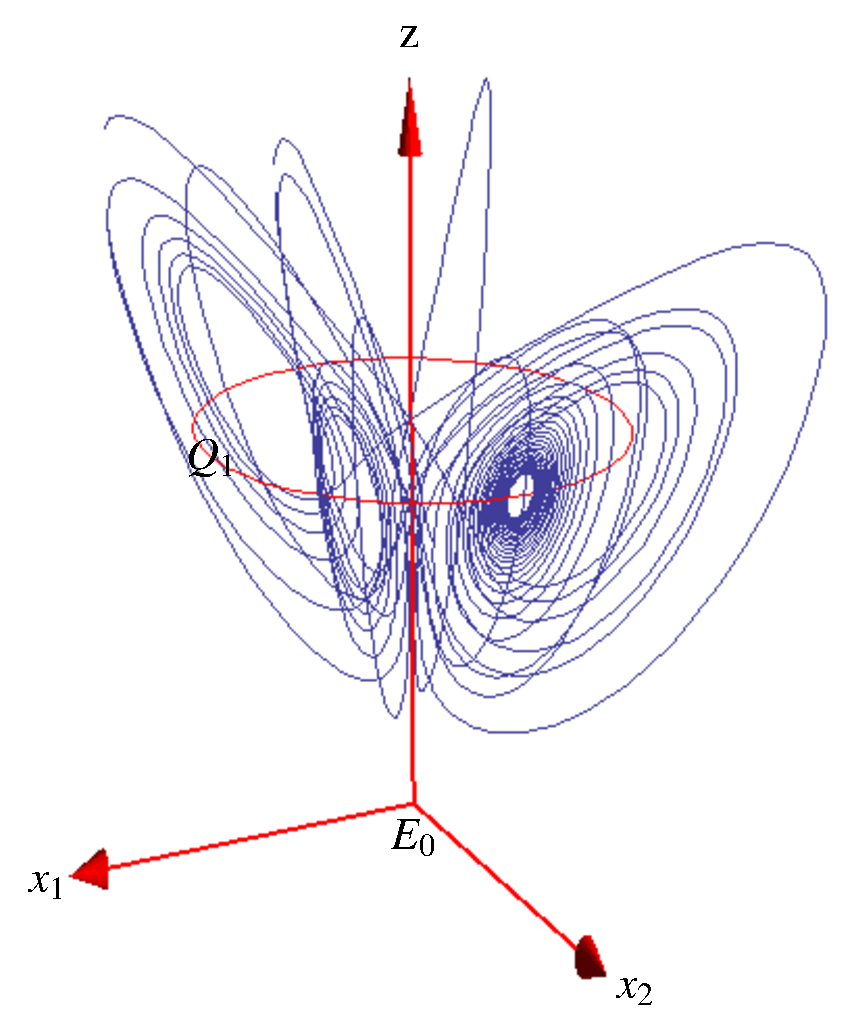
\includegraphics[width=0.35\textwidth, clip=true]{../figs/CLEtransv}
~~~~(\textit{b})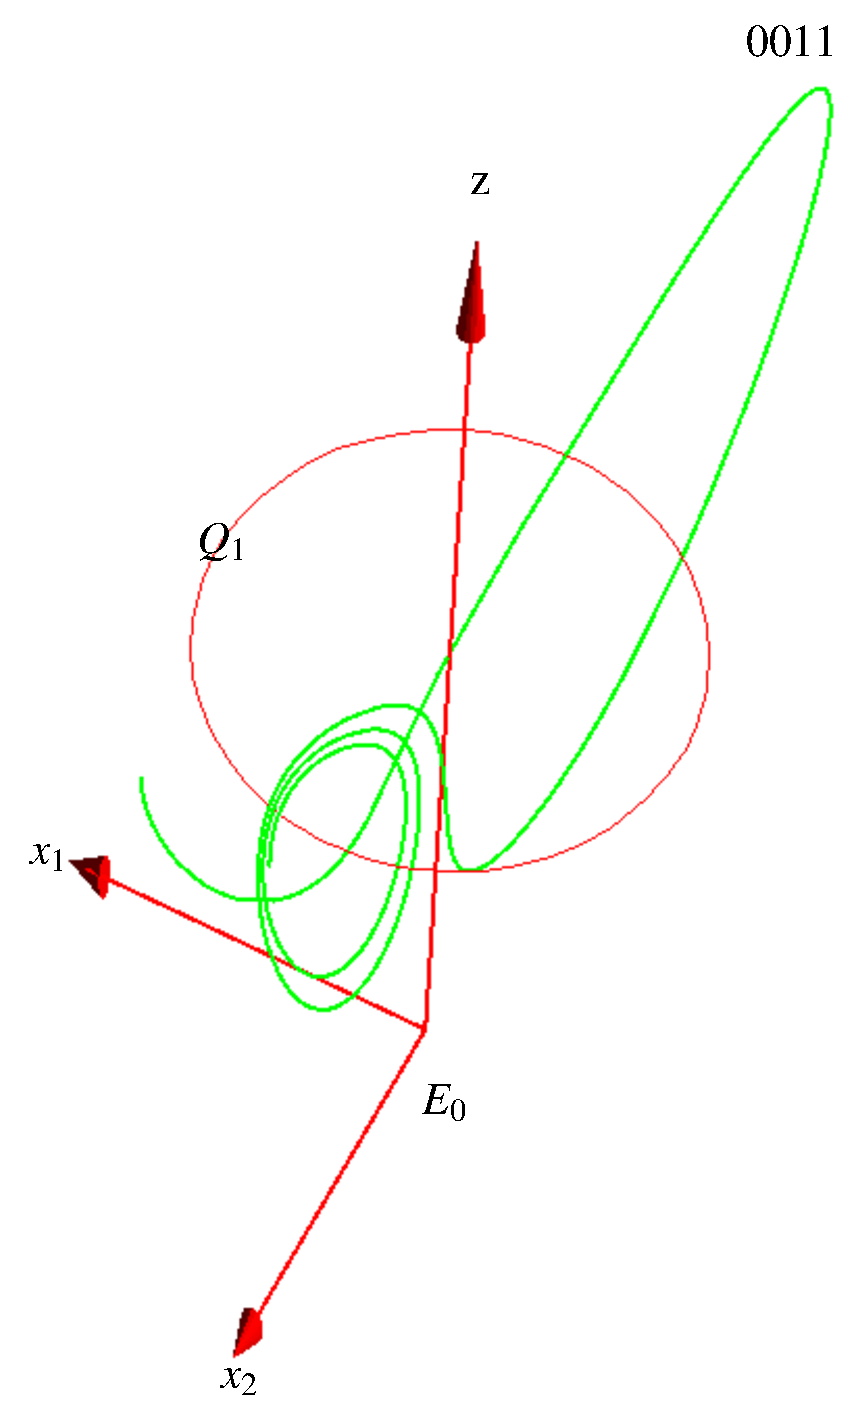
\includegraphics[width=0.35\textwidth, clip=true]{../figs/CLEtransvCyc}

\end{center}
\caption[\CLe\ desymmetrization with transverse integration]{
Attempt to restrict \CLe\ dynamics on the {\slice} $\mathcal{K}$ through
\refeq{eq:difeqTransv}. (a) A trajectory initiated on the unstable
manifold of $\REQV{}{1}$, (b) \rpo\ ``0011''
($e=1/10$, $\ImrCLor=0$).
    }
\label{fig:CLEtransv}
\end{figure}
%%%%%%%%%%%%%%%%%%%%%%%%%%%%%%%%%%%%%%%%%%%%%%%%%%%%%%%%%%%%%%%%

%%%%%%%%%%%%%%%%%%%%%%%%%%%%%%%%%%%%%%%%%%%%%%%%%%%%%%%%%%%%%%%%%%
\begin{figure}[ht]
\begin{center}
  (\textit{a})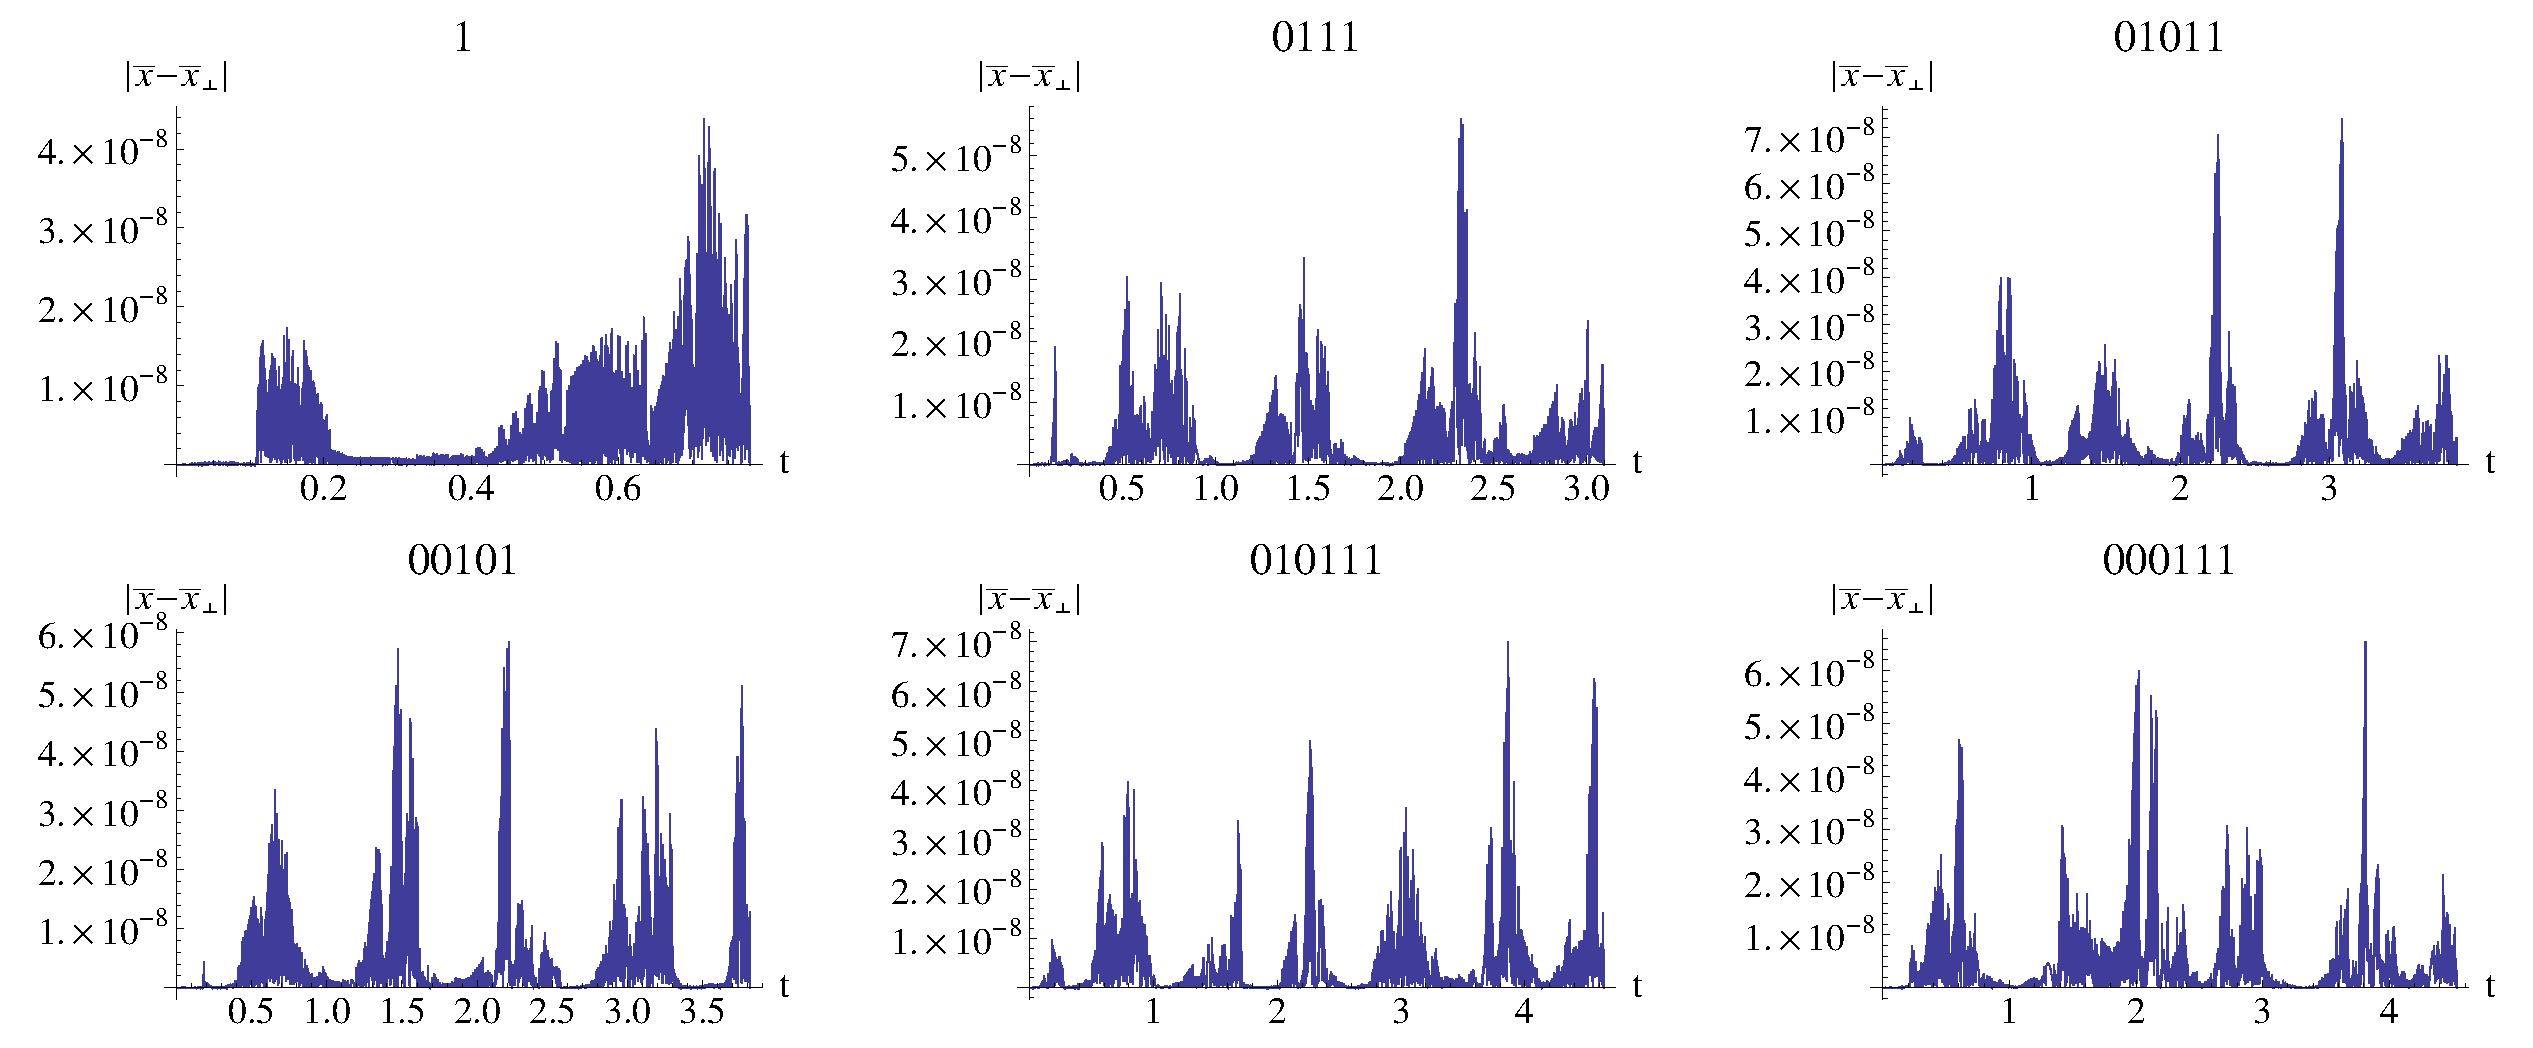
\includegraphics[width=0.9\textwidth, clip=true]{../figs/CLEerrTransv}
\end{center}
\caption[Numerical error in \CLe\ desymmetrization with transverse integration]{
Distance of $\ssp^\perp(t)$ to $\ssp(t)$ in invariant variables\refeq{eq:invLaser2}
for selected \rpo s of \CLe\,
($e=1/10$, $\ImrCLor=0$).
    }
\label{fig:CLEerrTransv}
\end{figure}
%%%%%%%%%%%%%%%%%%%%%%%%%%%%%%%%%%%%%%%%%%%%%%%%%%%%%%%%%%%%%%%%

In figure \reffig{fig:CLEerrTransv} we evaluate the accuracy
of integration of \refeq{eq:difeqTransv} by integrating
initial conditions for several \rpo s both in \statesp\ and
on the section and compute the distance
$|\overline{\ssp}(t)-\overline{\ssp}^\perp(t)|$ in invariant
variables \refeq{eq:invLaser2} (the norm is Euclidean). The
distance does not grow exponentially indicating that
numerical solution of \refeq{eq:difeqTransv} is accurate.
    \PC{\refFig{fig:CLEtransv} shows that there is something
    wrong with the way you implement dynamics within the
    {\slice}, as a relative periodic must surely close into a
    periodic one, as there is no motion in the translational
    direction. \refFig{fig:CLEerrTransv} shows that the error
    you make is only in the transverse direction, hence no
    significant error when you project it onto quotiented
    dynamics. {\bf PC Oct 2009:} in the above, I was wrong.
    Method of connections yields a geometric phase.}

\subsection{Integration on the {\slice} II}

    }%end ESedit
\PCedit{
Define the projection operator
\beq
 	\PperpOp_{ij}(\ssp_o)=\delta_{ij}-
    \frac{(\Lg \ssp_0)_i (\Lg \ssp_0)_j}{(\Lg \ssp_0)^2}
\ee{transvProj0}
that projects a $d$-dimensional flow $\vf(\ssp)$ onto
flow
\beq
	\dot{\ssp}_\perp = \vf_\perp(\ssp) = \vf(\ssp)
    - \Lg \ssp_0 \frac{(\Lg\ssp_0)\cdot\vf(\ssp)}{(\Lg \ssp_0)^2}
\ee{transvFlow}
in a $(d\!-\!1)$-dimensional {\slice} transverse to the
direction fixed by an arbitrary point $\ssp_0$.
       } % end PCedit
    \RLD{I think this way of removing SO(2) will only work if the
    {\slice} through $\ssp_0$ is flat, i.e. if the group action
    everywhere on the {\slice}  is parallel to $\Lg \ssp_0$.
    Therefore, I don't think this will work for KSE, where the
    $\pS/\SOn{2}$ manifold is not flat.  If the {\slice}  is not flat,
    then, once we move away from $\ssp_0$, the group action is
    not going to be in the direction of $\Lg \ssp_0$, so we will
    be projecting away the wrong direction, i.e. moving off the
    slice.  We would be able to stay on the slice if we kept
    updating the projector, i.e. use $\Lg x$ instead of $\Lg
    \ssp_0$, but in this case the accumulated phase shift would
    not be equal to the phase shift of an RPO.  See {\tt
    kse\_removing\_so2.pdf} in {\tt siminos/blog/davidchack/}.
    }
    \ES{Is what Ruslan describes in {\tt
    kse\_removing\_so2.pdf} a manifestation of what is
    called geometric phase in \rf{rowley_reduction_2003}? I
    believe this is the reason for failure in
    \reffig{fig:CLEtransv} but every time I mention it my
    former adviser tells me I read too much science fiction.}
If we replace our differential equations \refeq{eq:difeq}
with the system
\beq
	\frac{dx}{dt}=\PperpOp(x_o) v(x)\,,
	\label{eq:difeqTransvII}
\eeq
where $x_o$ a point on the {\slice}, solutions will stay on
the {\slice} $\mathcal{K}$ for any initial condition on
$\mathcal{K}$ as there is no component of $\PperpOp(x_o)
v(x)$ in the direction of the continuous symmetry. Note that
dynamics on the slice are equivariant under rotations by
$\pi$.


%%%%%%%%%%%%%%%%%%%%%%%%%%%%%%%%%%%%%%%%%%%%%%%%%%%%%%%%%%%%%%%%%%
\begin{figure}[ht]
\begin{center}
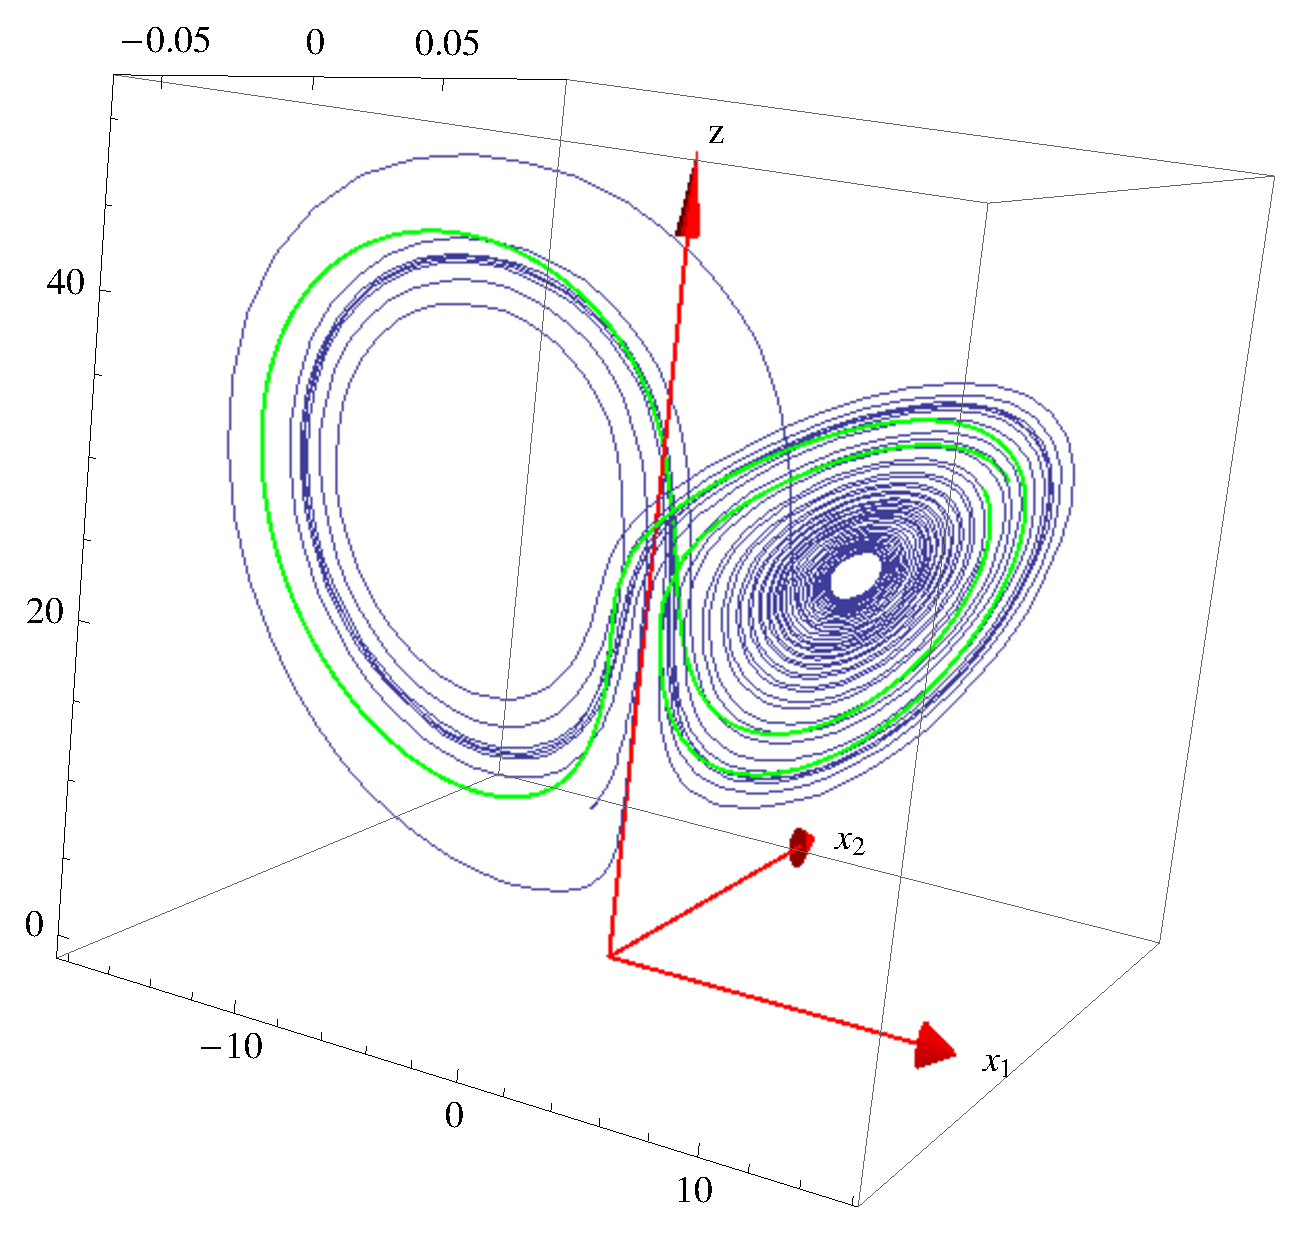
\includegraphics[width=0.5\textwidth, clip=true]{../figs/CLEtransvRPO}
\end{center}
\caption[\CLe\ desymmetrization with transverse integration II]{
Restriction of \CLe\ dynamics on the {\slice} $\mathcal{K}$ through
\refeq{eq:difeqTransvII}. A trajectory initiated on the unstable
manifold of $\REQV{}{1}$ is shown in blue and \rpo\ ``011'' is shown
in green.
($e=1/10$, $\ImrCLor=0$).
    }
\label{fig:CLEtransvII}
\end{figure}
%%%%%%%%%%%%%%%%%%%%%%%%%%%%%%%%%%%%%%%%%%%%%%%%%%%%%%%%%%%%%%%%
